% --- Template for thesis / report with tktltiki2 class ---
% 
% last updated 2013/02/15 for tkltiki2 v1.02

\documentclass[finnish]{tktltiki2}

% tktltiki2 automatically loads babel, so you can simply
% give the language parameter (e.g. finnish, swedish, english, british) as
% a parameter for the class: \documentclass[finnish]{tktltiki2}.
% The information on title and abstract is generated automatically depending on
% the language, see below if you need to change any of these manually.
% 
% Class options:
% - grading                 -- Print labels for grading information on the front page.
% - disablelastpagecounter  -- Disables the automatic generation of page number information
%                              in the abstract. See also \numberofpagesinformation{} command below.
%
% The class also respects the following options of article class:
%   10pt, 11pt, 12pt, final, draft, oneside, twoside,
%   openright, openany, onecolumn, twocolumn, leqno, fleqn
%
% The default font size is 11pt. The paper size used is A4, other sizes are not supported.
%
% rubber: module pdftex

% --- General packages ---

\usepackage[utf8]{inputenc}
\usepackage[T1]{fontenc}
\usepackage{lmodern}
\usepackage{microtype}
\usepackage{amsfonts,amsmath,amssymb,amsthm,booktabs,color,enumitem,graphicx}
\usepackage{gensymb}
\usepackage[pdftex,hidelinks]{hyperref}

\usepackage{pgf,tikz}
\usepackage{tkz-euclide}
\usetikzlibrary{arrows, babel, calc, quotes}
\usetkzobj{all}

% Automatically set the PDF metadata fields
\makeatletter
\AtBeginDocument{\hypersetup{pdftitle = {\@title}, pdfauthor = {\@author}}}
\makeatother

% --- Language-related settings ---
%
% these should be modified according to your language

% babelbib for non-english bibliography using bibtex
\usepackage[fixlanguage]{babelbib}
\selectbiblanguage{finnish}

% add bibliography to the table of contents
\usepackage[nottoc]{tocbibind}
% tocbibind renames the bibliography, use the following to change it back
\settocbibname{Lähteet}

% --- Theorem environment definitions ---

\newtheorem{lau}{Lause}
\newtheorem{lem}[lau]{Lemma}
\newtheorem{kor}[lau]{Korollaari}

\theoremstyle{definition}
\newtheorem{maar}[lau]{Määritelmä}
\newtheorem{ong}{Ongelma}
\newtheorem{alg}[lau]{Algoritmi}
\newtheorem{esim}[lau]{Esimerkki}

\theoremstyle{remark}
\newtheorem*{huom}{Huomautus}


% --- tktltiki2 options ---
%
% The following commands define the information used to generate title and
% abstract pages. The following entries should be always specified:

\title{Valaistusmallinnus reaaliaikaisessa 3D-grafiikassa}
\author{Miko Mynttinen}
\date{\today}
\level{Kandidaatintutkielma}
\abstract{Tässä tutkielmassa tarkastellaan reaaliaikaisen kolmiulotteisen tietokonegrafiikan mallinnusta, renderöinnin toteutusta piirtoliukuhihnamallilla, ja valaistusmallinnusta. Valaistusmalleista tarkastellaan erityisesti Phongin valaistusmallia, jonka fysikaalinen perusta käydään läpi ja siitä johdetaan valaistusyhtälö. Valaistusyhtälö evaluoidaan tietokoneohjelmalla samalle monikulmiomallille kolmella eri varjostustekniikalla: tasaisella, Gouraudin ja Phongin varjostuksella. Tuloksena saatuja kuvia vertaillaan ja huomataan, että tasaisella varjostuksella kappaletta mallintava monikulmioverkko jää näkyviin. Gouraudin varjostus ratkaisee tämän ongelman mattapinnoilla, mutta sen heikkous spekulaarisesti heijastavilla pinnoilla motivoi Phongin varjostuksen käyttöön. Phongin varjostuksella valaistusmallin spekulaarisen heijastuman vaimeneminen näyttää tasaiselta ja lopputulos on todenmukaisuudeltaan tyydyttävä.}

% The following can be used to specify keywords and classification of the paper:

\keywords{valaistus, varjostus, tietokonegrafiikka}

% classification according to ACM Computing Classification System (http://www.acm.org/about/class/)
% This is probably mostly relevant for computer scientists
% uncomment the following; contents of \classification will be printed under the abstract with a title
% "ACM Computing Classification System (CCS):"
\classification{
\textbf{Computing methodologies $\rightarrow$ Rendering}\\
\textbf{Computing methodologies $\rightarrow$ Reflectance modeling}
}

% If the automatic page number counting is not working as desired in your case,
% uncomment the following to manually set the number of pages displayed in the abstract page:
%
% \numberofpagesinformation{16 sivua + 10 sivua liitteissä}
%
% If you are not a computer scientist, you will want to uncomment the following by hand and specify
% your department, faculty and subject by hand:
%
% \faculty{Matemaattis-luonnontieteellinen}
% \department{Tietojenkäsittelytieteen laitos}
% \subject{Tietojenkäsittelytiede}
%
% If you are not from the University of Helsinki, then you will most likely want to set these also:
%
% \university{Helsingin Yliopisto}
% \universitylong{HELSINGIN YLIOPISTO --- HELSINGFORS UNIVERSITET --- UNIVERSITY OF HELSINKI} % displayed on the top of the abstract page
% \city{Helsinki}
%

% Riviväli
\usepackage[nodisplayskipstretch]{setspace}
%\singlespacing
%\onehalfspacing
\doublespacing

\begin{document}

% --- Front matter ---

\frontmatter      % roman page numbering for front matter

\maketitle        % title page
\makeabstract     % abstract page

\tableofcontents  % table of contents

% --- Main matter ---

\mainmatter       % clear page, start arabic page numbering

% Write some science here.
\section{Johdanto}
Kolmiulotteisella tietokonegrafiikalla tarkoitetaan kuvien tuottamista tietokoneella käyttäen lähteenä kolmiulotteisia malleja. Tässä tutkielmassa käsitellään etenkin reaaliaikaisessa kolmiulotteisessa tietokonegrafiikassa käytettäviä tekniikoita. Reaaliaikaisuus tarkoittaa, että kuvia tuotetaan yli 30 kuvaa sekunnissa. Tämä asettaa rajoituksia käytettävien tekniikoiden aikavaatimuksiin.

Tietokonegrafiikalla pyritään usein tuottamaan todenmukaisia kuvia, joten käytettävät tekniikat perustuvat yleensä luonnon toiminnan mallintamiseen. Näistä tekniikoista etenkin valaistusmallinnuksella on suuri vaikutus tuotettujen kuvien todenmukaisuuden vaikutelmaan, koska kaikki näkeminen perustuu valon heijastumiseen~\cite[s. 101-113]{Hughes}. Tässä tutkielmassa tarkastellaan yleisesti käytettyä Phongin valaistusmallia ja vertaillaan kuinka erilaiset tavat käyttää tätä valaistusmallia vaikuttavat lopputuloksena saatavan kuvan laatuun.

Tutkielman rakenne etenee seuraavasti. Luvussa 2 tutustutaan kolmiulotteisen tietokonegrafiikan ja valaistusmallinnuksen perusteisiin ja toteutukseen nykyaikaisilla näytönohjaimilla. Luvussa 3 tarkastellaan Phongin valaistusmallia. Valaistusmallin fysikaalinen perusta käydään läpi ja siitä johdetaan valaistuksessa käytettävä matemaattinen malli eli valaistusyhtälö. Luvussa 4 tutustutaan tapoihin evaluoida valaistusyhtälö kuvan pikseleille ja vertaillaan näiden vaikutusta tuotettujen kuvien todenmukaisuuteen.

\newpage
\section{Kolmiulotteinen tietokonegrafiikka}
Kuvan tuottamista kolmiulotteisesta mallista kutsutaan renderöinniksi. Näkymän renderöinti tapahtuu projisoimalla mallinnettu kolmiulotteinen maailma kaksiulotteiselle tasolle. Tätä voidaan ajatella siten, että mallinnetusta maailmasta otetaan virtuaalisella kameralla valokuva.

Tässä luvussa käsitellään ensin tapoja mallintaa kolmiulotteista maailmaa ja sen valaistusta, jonka jälkeen käydään läpi renderöinnin eri vaiheet ja niiden toteutus näytönohjaimella.

\subsection{Kolmiulotteisen tietokonegrafiikan mallinnus}
Kolmiulotteisen tietokonegrafiikan maailma on kokoelma malleja, jotka kuvaavat siinä olevia kappaleita. Eräs yksinkertainen malli on lista kolmiulotteisen avaruuden pisteitä, joista jokainen kolmen peräkkäisen pisteen joukko tulkitaan kolmion määrittävien kulmapisteiden joukkona. Tämä onkin nykyään yleisin tapa mallintaa kappaleita, sillä useimmat reaaliaikaista tietokonegrafiikkaa tuottavat järjestelmät odottavat syötteenä annettujen mallien koostuvan kolmioista~\cite[s. 8]{Moller}. Pisteitä, janoja ja kolmioita kutsutaan usein piirtoprimitiiveiksi, koska monimutkaisemmat kappaleet mallinnetaan niiden yhdistelmillä. Esimerkiksi suorakulmio saadaan rakennettua neljästä kulmapisteestä, joista muodostetaan kaksi kolmiota yhdellä jaetulla sivulla. Kuvassa~\ref{fig:Monikulmioverkko}\footnote{Kuvat on tuotettu C++-kielellä ohjelmoidulla tietokoneohjelmalla.} havainnollistetaan kolmioverkolla mallinnettua palloa. Myös muunlaiset monikulmioverkot ovat yleisesti käytössä ja esimerkiksi nelikulmioita käytetään usein kolmiulotteisten mallinnusohjelmien kanssa~\cite[s. 636]{Hughes}. Nämä monikulmioverkot voidaan kuitenkin edelleen jakaa kolmioverkoiksi, joten tässä tutkielmassa käytetään kolmion ja kolmioverkon sijasta usein myös termejä monikulmio ja monikulmioverkko.

\begin{figure}[h]
\centering
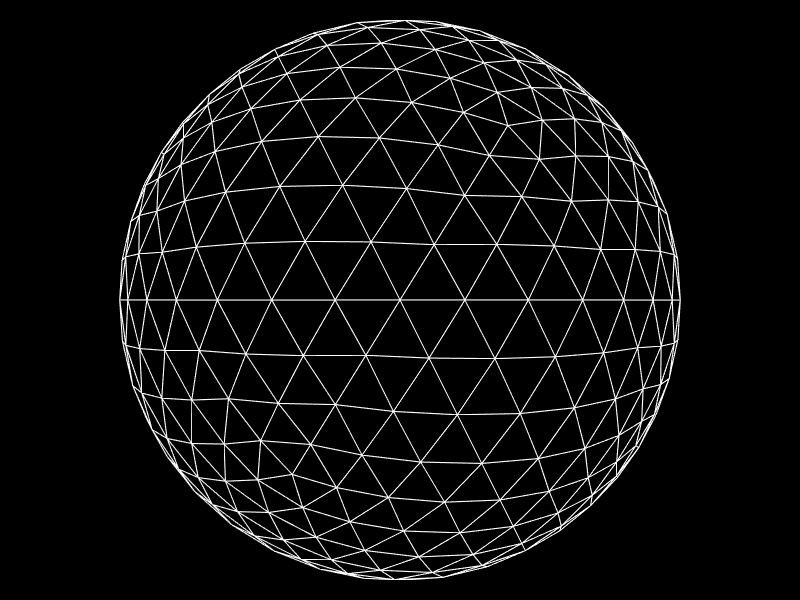
\includegraphics[scale=0.6]{img/wireframe_crop.png}
\caption{Kolmioista muodostettu pallo.}
\label{fig:Monikulmioverkko}
\end{figure}

Yhtälöihin perustuvat mallit voivat kuvata esimerkiksi käyriä tai pintoja. Kun kappaleen määrittämä yhtälö evaluoidaan halutuilla arvoilla kuten skaalauskertoimella ja sijainnilla, saadaan tuloksena kappaleen määrittävät pisteet. Kun pisteet tulkitaan janojen päätepisteinä, saadaan renderöityä käyrä. Saadut pisteet voidaan myös tulkita monikulmioina, jotka kolmioidaan eli jaetaan kolmioiksi, ja renderöidään pintoina.

Näkymän kolmiulotteisiin malleihin liitetään usein myös muuta tietoa kuten tekstuureja, joita voidaan ajatella kappaleen päälle liimattavina kuvina. Tekstuureja käytetään esimerkiksi kappaleen pinnan materiaalin määrittämiseen ja kuvien esittämiseen kappaleen pinnalla. Tekstuureja käytettäessä liitetään malliin yleensä myös tekstuurikoordinaatit, joilla määritetään tekstuurin sijainti kappaleen pinnalla.

Muuta malleihin usein sisällytettävää tietoa ovat kulmapisteisiin liitetyt kulmapistenormaalit. Kulmapistenormaali on kulmapistettä ympäröivien pintojen normaalivektorien normalisoitu keskiarvo. Kulmapistenormaalia havainnollistetaan kuvassa~\ref{fig:Kulmapistenormaali}.
\begin{figure}[h]
\centering
\begin{tikzpicture}[line cap=round,line join=round,>=triangle 45,x=1.0cm,y=1.0cm]
\clip(-2.0, -1.0) rectangle (2.0, 2.0);

\coordinate (A) at (-1.0, -1.0);
\coordinate (B) at (1.0, -1.0);
\coordinate (O) at (0.0, 0.0);

\draw[red,->] (-0.5, -0.5) -- ($(-0.5, -0.5)!1cm!(-1.0, 0.0)$);
\draw[green,->] (0.5, -0.5) -- ($(0.5, -0.5)!1cm!(1.0, 0.0)$);
\draw[yellow,->] (0.0, 0.0) -- ($(0.0, 0.0)!1cm!(0.0, 1.0)$);

\draw[-] (O) -- (A);
\draw[-] (O) -- (B);

\fill (0.0, 0.0) circle[radius=2pt];

\begin{normalsize}
\draw[color=black] (0.0, -0.4) node {$\vec{v}$};

\draw[color=black] (0.0, 1.3) node {$\vec{N_v}$};
\draw[color=black] (-1.5, 0.5) node {$\vec{N_1}$};
\draw[color=black] (1.5, 0.5) node {$\vec{N_2}$};
\end{normalsize}
\end{tikzpicture}

\caption{Kahden pinnan normaalivektorit $\vec{N_1}$ ja $\vec{N_2}$, pintojen jakama kulmapiste $\vec{v}$, ja kulmapistenormaali $\vec{N_v}$.}
\label{fig:Kulmapistenormaali}
\end{figure}

\subsection{Valaistusmallinnus}
Valaistusmallinnus tarkoittaa valojen ja varjojen simulointia empiirisillä tai fysiikkaan perustuvilla matemaattisilla malleilla. Näillä malleilla kolmiulotteiseen maailmaan voidaan sijoittaa valonlähteitä, joista lähtevän valon vaikutukset näkyvät kappaleiden pintojen kirkkauden ja värin muutoksina. Valaistusmallit pyrkivät mallintamaan valon käyttäytymistä luonnossa: kappaleet, joihin ei osu valoa eivät näy, ja kappaleet joihin osuu valoa, näkyvät vaihtelevalla kirkkaudella riippuen valonlähteiden määrästä, sijainnista ja kirkkaudesta. Kappaleen kirkkauden ja värin lisäksi valaistusmallit mallintavat kappaleiden materiaaleja. Materiaalit määrittävät esimerkiksi kappaleen heijastavuuden.

Mikäli valaistusmallinnusta ei olisi, ei kuvissa näkyisi varjoja ja kappaleet näyttäisivät tasaisen mattapintaisilta ja litteiltä. Kuvassa~\ref{fig:Ambient} havainnollistetaan kolmiulotteista mallia, joka on renderöity tasaisella värillä ilman valaistusmallinnusta. Kuvasta nähdään kuinka pallon syvyysvaikutelma katoaa täysin. Valaistusmallinnus on siis tärkeä osa realismiin pyrkivää tietokonegrafiikkaa.
\begin{figure}[h]
\centering
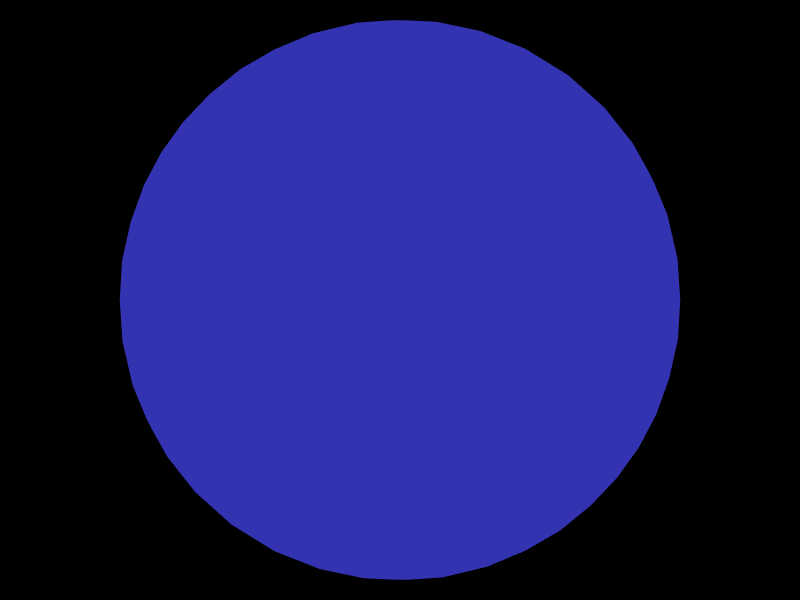
\includegraphics[scale=0.6]{img/ambient_crop.png}
\caption{Tasaisella värillä renderöity pallo.}
\label{fig:Ambient}
\end{figure}

Valaistusmallit voidaan jakaa karkeasti kahteen luokkaan: paikallisiin ja globaaleihin valaistusmalleihin. Paikallisilla valaistusmalleilla simuloidaan vain valonlähteestä suoraan kappaleen pinnan pisteisiin osuvaa valoa, eli valon heijastumista pintojen välillä ei oteta huomioon. Globaalit valaistusmallit mallintavat näiden lisäksi myös valon heijastumista pintojen välillä ja ovat täten  laskennallisesti paljon vaativampia. Täysin globaaleja valaistusmalleja käytetään harvemmin reaaliaikaisessa tietokonegrafiikassa, jonka vuoksi tässä tutkielmassa keskitytään lokaaleihin valaistusmalleihin.

Valaistusmallilla tarkoitetaan valon käyttäytymisen mallia ja siitä johdettua valaistusyhtälöä. Valaistusyhtälö määrittää kappaleen pinnan yksittäisen pisteen heijastaman valon määrän eli pisteen kirkkauden.

Pisteen kirkkautta kutsutaan etenkin vanhemmissa tietokonegrafiikan artikkeleissa intensiteetiksi, mutta nykyään tarkempien fysiikkaan perustuvien valaistusmallien yhteydessä radianssi on täsmällisempi termi~\cite[s. 700]{Hughes}. Radianssi on radiometrian suure, joka kuvaa pinnalta heijastuvan säteilyn määrää. Koska tässä tutkielmassa käsitellään klassisia ja osittain empiirisiä valaistusmalleja, käytetään termiä intensiteetti. Harmaasävykuvia käsitellessä intensiteetin voidaan ajatella olevan liukuluku välillä $[0, 1]$, missä arvo $0.0$ vastaa mustaa ja $1.0$ valkoista. Värien esittämiseen tietokonegrafiikassa käytetään yleensä punaisesta, vihreästä ja sinisestä väristä koostuvia RGB-kolmikoita, jotka 24-bittisillä väreillä rajoitetaan välille $[0, 255]$. Eräs keino mallintaa värikuvien valaistusta on skalaarikertolasku. Olkoon pikselin $P$ alkuperäinen väriarvo $c = (r, g, b)$. Pikselin lopullinen väriarvo saadaan kertomalla kolmikko valaistusyhtälöstä saadulla intensiteetillä $I$, eli $I_P = I\cdot c = (Ir, Ig, Ib)$.

Pinnan pisteen tai pikselin värin määritystä valaistusyhtälön avulla kutsutaan varjostamiseksi, jota käsitellään luvussa~\ref{sec:Varjostus}.

\subsection{Piirtoliukuhihna}
Kolmiulotteisen kuvan tuottamisen voidaan ajatella tapahtuvan yhteen suuntaan kulkevalla liukuhihnalla, jonka jokainen vaihe tuottaa ulostulona seuraavan vaiheen syötteen. Tässä käsiteltävä yksinkertaistettu piirtoliukuhihna määritellään Akenine-Möllerin ja kumppanien mallin~\cite[s. 11-27]{Moller} mukaisesti. Tämä malli jakaa liukuhihnan kolmeen vaiheeseen: sovellus-, geometria- ja rasterointivaiheisiin. On tärkeää huomata että tämä on vain korkean tason käsitteellinen jako ja varsinaiset ohjelmisto- ja laitteistototeutukset ovat monimutkaisempia. Seuraavassa luvussa käsitellään miten tämä piirtoliukuhihnan malli on toteutettu nykyaikaisilla näytönohjaimilla.

Nykyaikaisissa tietokonejärjestelmissä renderöinti aloitetaan yleensä keskussuorittimella ajettavalla sovellusvaiheella, jonka jälkeen geometria- ja rasterointivaiheet suoritetaan näytönohjaimella. Sovellusvaiheessa grafiikkaohjelmisto valmistelee tietokoneen näytönohjaimen renderöintiä varten. Ohjelmisto myös siirtää näytönohjaimen muistiin renderöinnissä tarvittavat tiedot kuten kappaleiden kolmioiden kulmapistetiedot ja tekstuurit. 

Geometriavaiheessa suoritetaan kulmapiste- ja kolmiokohtaiset operaatiot kuten näkymän kolmioiden kulmapisteiden kääntö, siirto ja skaalaus. Muita tässä vaiheessa suoritettavia tehtäviä ovat projektio- ja perspektiivimuunnokset, joilla kolmiulotteinen näkymä rajataan ja kuvataan kaksiulotteiselle tasolle.

Rasterointivaiheessa kuvan jokaisen pikselin väriarvo tallennetaan näytönohjaimen väripuskuriin. Väripuskuri on näytönohjaimen muistissa sijaitseva taulukko, joka sisältää pikseleiden värin punaisen, vihreän ja sinisen komponentin kolmikkona. Pikseleiden värit määräytyvät sen kolmion mukaan, minkä alueelle pikselit jäävät. Mikäli pikseli jää usean kolmion alueelle, määritetään väri käyttämällä kolmioiden syvyystietoja, joiden avulla pikselille valitaan päällimmäisenä olevan kolmion väri. Mikäli kolmiolle on määritelty tekstuuri, haetaan pikselin väriarvo tekstuurista tekstuurikoordinaattien mukaisesti. Rasterointivaiheen jälkeen näytönohjaimen väripuskuri voidaan siirtää kuvaruudulle tai esimerkiksi tallentaa tiedostoksi.

\subsection{Näytönohjaimet}
Nykyään yleisin tapa tuottaa reaaliaikaista kolmiulotteista tietokonegrafiikkaa on käyttää grafiikkaan ja rinnakkaislaskentaan suunniteltua näytönohjainta, joka sisältää yhden tai useamman grafiikkasuorittimen~\cite[s. 18]{Hughes}. Tärkeimmät syyt grafiikkasuoritinten käyttöön tietokonegrafiikassa ovat renderöinnin tehokas rinnakkaistuvuus pikseli- ja monikulmiotasolla~\cite{Crockett}, ja grafiikkasuoritinten optimointi etenkin grafiikkalaskennassa käytettyihin laskutoimituksiin, kuten skalaarien ja vektorien kerto- ja yhteenlaskuun ja näiden yhdistelmiin~\cite[s. 32]{Moller}.

Nykyaikaiset grafiikkasuorittimet koostuvat jopa tuhansista monikäyttöisistä suoritinytimistä, joita kutsutaan ohjelmoitaviksi varjostinyksiköiksi. Varjostinyksiköillä voidaan suorittaa varjostinohjelmointiin tarkoitetuilla ohjelmointikielillä kirjoitettuja varjostinohjelmia eli varjostimia. Varjostimet on kehitetty piirtoliukuhihnan eri vaiheiden toteuttamiseen laitteistotasolla siten, että käyttäjä voi ohjelmoimalla muuttaa näytönohjaimen piirtoliukuhihnan toimintaa~\cite[s. 927-931]{Hughes}.

Piirtoliukuhihnan kannalta kaksi tärkeintä varjostinta ovat kulmapistevarjostin, joka suorittaa piirtoliukuhihnan kulmapistekohtaiset operaatiot, ja pikselivarjostin, joka suorittaa pikselikohtaiset operaatiot. Nämä varjostimet siis suorittavat piirtoliukuhihnan geometria- ja rasterointivaiheiden toiminnot. 

Grafiikkaohjelmisto syöttää kulmapistetiedot ensimmäisenä kulmapistevarjostimelle, joka suoritetaan kerran jokaiselle näkymän kulmapisteelle. Kulmapisteet muunnetaan ohjelmoijan määrittämällä tavalla, jonka jälkeen niitä käytetään mallien piirtoprimitiivien piirtämiseen. Kulmapistevarjostimen ulostulo syötetään pikselivarjostimelle pikselikohtaisesti interpoloituna~\cite[s. 935-939]{Hughes}, joka on hyödyllistä esimerkiksi luvussa~\ref{sec:Varjostus} käsiteltävän Gouraudin ja Phongin varjostuksen toteuttamisessa.

Pikselivarjostin ajetaan kulmapistevarjostuksen jälkeen näkymän piirtoprimitiivien alueille jääville pikseleille. Pikselivarjostimen ulostulona saadaan pikselin väriarvo ja se kirjoitetaan usein suoraan näytönohjaimen väripuskuriin. 

\newpage
\section{Phongin valaistusmalli}
Phongin valaistusmalli on Bui-Tuong Phongin~\cite{Phong} vuonna 1975 kehittämä paikallinen valaistusmalli. Phongin kehittämällä valaistusmallilla voidaan laskea valon intensiteetti pinnan pisteessä, kunhan tiedetään katsojan, pinnan pisteen ja valonlähteen suhteelliset sijainnit. Pinnan materiaalin heijastavuutta ja valon ominaisuuksia voidaan muuttaa mallin vakiokertoimien avulla.

Tässä luvussa käsitellään valaistusmallin fysikaalinen perusta, josta johdetaan valaistusyhtälö. Lisäksi esitellään yleisesti käytetty valaistusmallin laskennallisesti helpompi muunnelma.

\subsection{Fysikaalinen perusta}
Tämä käsittely pohjautuu Antti Puhakan kirjan \textit{3D-grafiikka}~\cite{Puhakka} lukuun 11.

Phongin empiirisessä mutta osittain fysiikkaan perustuvassa mallissa pinnan pisteeseen osuvan valon intensiteetin voidaan ajatella koostuvan kolmesta eri komponentista: taustavalosta, diffuusisti heijastuvasta valosta ja spekulaarisesti heijastuvasta valosta.

Diffuusi heijastuminen tarkoittaa valonlähteestä saapuvan valonsäteen heijastumista pinnan pisteestä kaikkiin suuntiin tasaisesti. Diffuusia heijastumista voidaan mallintaa termillä
\begin{align*}
I = k_dI_p\,,
\end{align*}
missä $I$ on pinnasta heijastuvan valon intensiteetti, $k_d$ on pinnan diffuusin heijastumisen kerroin ja $I_p$ on pintaan osuvan valon intensiteetti.

Pistemäistä ja äärettömän kaukana sijaitsevaa valonlähdettä voidaan mallintaa siten, että kaikilla valonlähteestä lähtevillä valonsäteillä ajatellaan olevan sama suuntavektori. Jos tiedetään pinnan normaalivektori $\vec{N}$, valonlähteeseen osoittava suuntavektori $\vec{L}$ ja näiden välinen kulma $\theta$, voidaan pinnalta heijastuvan valon intensiteetti laskea Lambertin kosinilailla.
Lambertin kosinilain mukaan pinnalta heijastuvan valon intensiteetti riippuu valonlähteen suuntavektorin ja pinnan normaalivektorin kulman kosinista. Tämä tarkoittaa, että valon intensiteetti on pienimmillään kun kulma on 90 astetta ja suurimmillaan kun kulma on 0 astetta. Lambertin lakia havainnollistetaan kuvassa~\ref{fig:Lambertin_laki}, missä pinnalla alueelle $d$ saapuu valonsäteitä tapauksissa $\theta = 0\degree$ (vasemmalla) ja $\theta = 45\degree$ (oikealla). 
\begin{figure}[h]
\centering
\begin{tikzpicture}[line cap=round,line join=round,>=triangle 45,x=1.0cm,y=1.0cm]
\clip(-4.0, -0.5) rectangle (4.0, 3.0);

\coordinate (O) at (1.0, 0.0);
\coordinate (N) at (1.0, 3.0);

\coordinate (A) at (2.0, 1.0);
\coordinate (B) at (3.0, 0.0);
\coordinate (C) at (1.0, 2.0);

\draw [->] (O) -- (N);
\draw [-] (A) -- (B);
\draw [-] (A) -- (O);

\draw [->] (2, 1) -- (4, 3);
\draw [->,yellow] (2.35, 0.65) -- (4, 23/10);
\draw [->,yellow] (2.7, 0.3) -- (4, 8/5);
\draw [->] (3, 0) -- (4, 1);

\coordinate (O2) at (-1.0, 0.0);
\coordinate (N2) at (-1.0, 3.0);

\coordinate (A2) at (-1.0, 1.0);
\coordinate (B2) at (-3.0, 1.0);
\coordinate (C2) at (-3.0, 0.0);

\draw [->] (O2) -- (N2);
\draw [-] (A2) -- (B2);
\draw [->] (-3.0, 0.0) -- (-3.0, 3.0);
\draw [->, yellow] (-2.5, 1.0) -- (-2.5, 3.0);
\draw [->, yellow] (-2.0, 1.0) -- (-2.0, 3.0);
\draw [->, yellow] (-1.5, 1.0) -- (-1.5, 3.0);

\draw [-] (-4, 0) -- (-1, 0);
\draw [-] (1.0, 0) -- (4, 0);

\tkzMarkAngle[thin, size=0.5](A,B,O);
\tkzLabelAngle[pos=0.7](A,B,O){$\theta$}
\tkzMarkAngle[thin, size=0.5](A,O,C);
\tkzLabelAngle[pos=0.7](A,O,C){$\theta$}

\tkzMarkRightAngle[thin, size=0.2](O,A,B)

%\tkzLabelAngle[pos=0.5](O2,C2,B2){$\theta$}
%\tkzMarkRightAngle[thin, size=0.2](O2,C2,B2)

\begin{small}
\draw[color=black] (3.5, 1.5) node {$\vec{L}$};
\draw[color=black] (0.8, 2.0) node {$\vec{N}$};
\draw[color=black] (2.0, -0.3) node {$d$};
\draw[color=black] (2.7, 0.7) node[rotate=-45] {$d\cos\theta$};

\draw[color=black] (-2.0, 2.5) node {$\vec{L}$};
\draw[color=black] (-0.8, 2.0) node {$\vec{N}$};
\draw[color=black] (-2.0, -0.3) node {$d$};
\draw[color=black] (-2.0, 1.2) node {$d\cos\theta$};
\end{small}

\end{tikzpicture}
\caption{Lambertin kosinilaki. Kuvassa $d$ on alueen pinta-ala, $\vec{L}$ valonlähteen suuntavektori, $\vec{N}$ pinnan normaalivektori ja $\theta$ näiden vektoreiden välinen kulma.}
\label{fig:Lambertin_laki}
\end{figure}\\
Kuvasta nähdään, että vasemmalla valonsäteiden poikkipinta-ala on pienempi joten pinnalle saapuu enemmän valonsäteitä ja täten pintaan osuvan valon intensiteetti on korkeampi. Pinnalle saapuvan valon intensiteetti riippuu siis kertoimesta $\cos\theta$ ja pinnalta heijastuvan valon intensiteetti voidaan laskea kaavalla
\begin{align}
\label{Lambert}
I = k_dI_p\cos\theta\,.
\end{align}
Kun pinnan normaalivektori $\vec{N}$ ja valonlähteeseen osoittava suuntavektori $\vec{L}$ oletetaan normalisoiduiksi, voidaan kaava~\ref{Lambert} kirjoittaa muodossa
\begin{align*}
I = k_dI_p\vec{N}\cdot\vec{L}\,.
\end{align*}

Taustavalo tarkoittaa valoa joka on peräisin pintojen välisistä heijastumista. Tällaisen valon tarkka mallinnus on sekä fysikaalisesti että laskennallisesti vaikeaa, joten taustavaloa mallinnetaan  usein vakiotermillä
\begin{align*}
\text{taustavalon termi} = k_dI_a\,,
\end{align*}
missä $k_d$ on pinnan diffuusin heijastumisen kerroin ja $I_a$ taustavalon intensiteetti. Vaikka tämän mallin mukaisesti myös taustavalo on pinnasta diffuusisti heijastuvaa valoa, voidaan taustavalon käyttäytymistä tarvittaessa muuttaa korvaamalla kerroin $k_d$ taustavalon diffuusin heijastumisen kertoimella $k_a$.

Spekulaaria heijastumista tapahtuu kiiltävillä pinnoilla, joilla osa valonlähteestä tulevasta valosta heijastuu pinnalta katsojaa kohti voimakkaammin kuin pelkästään diffuusista heijastumisesta. Tällaista heijastumista esiintyy esimerkiksi muovi-, lasi- ja metallipinnoilla.

Spekulaarin heijastumisen mallissa pinnan oletetaan olevan epätäydellinen peilipinta, eli että täydellisestä peilipinnasta poiketen valo heijastuu myös muihin suuntiin kuin täydelliseen heijastussuuntaan $\vec{R}$. Muihin suuntiin heijastuvan valon oletetaan vaimenevan.

Täydellinen heijastussuunta $\vec{R}$ voidaan laskea peilaamalla normalisoitu saapuvan valon valonlähteen suuntavektori $\vec{L}$ normalisoidun pinnan normaalivektorin $\vec{N}$ suhteen kaavalla
\begin{align*}
\vec{R} = 2(\vec{L}\cdot\vec{N})\vec{N} - \vec{L}\,.
\end{align*}

Phongin valaistusmallissa spekulaaristi heijastuva valo vaimenee täydellisen heijastussuunnan vektorin $\vec{R}$ ja katsojaan päin osoittavan suuntavektorin $\vec{V}$ välisen kulman $\alpha$ mukaan kertoimella $(\cos\alpha)^n$. Eksponentti $n$ määritetään empiirisesti ja se kuvaa pinnan heijastuksen vaimenemisen voimakkuutta. Suurempi eksponentti mallintaa nopeampaa vaimenemista. Näitä vektoreita ja kulmaa $\alpha$ havainnollistetaan kuvassa~\ref{fig:Phong_suuntavektorit}.

\begin{figure}[h]
\centering
\begin{tikzpicture}[line cap=round,line join=round,>=triangle 45,x=1.0cm,y=1.0cm]
\clip(-2.5, -0.1) rectangle (2.5, 2.5);

\coordinate (O) at (0.0, 0.0);
\coordinate (N) at (0.0, 1.0);
\coordinate (L) at (-3.0, 1.5);
\coordinate (V) at (2.0, 2.0);
\coordinate (R) at (3.0, 1.5);

\draw[->] (O) -- ($(O)!2cm!(R)$);
\draw[->] (O) -- ($(O)!2cm!(L)$);
\draw[->] (O) -- ($(O)!2cm!(V)$);
\draw[->] (O) -- ($(O)!2cm!(N)$);

\draw [-] (-2.5, 0) -- (2.5, 0);

\tkzMarkAngle[thick, size=1.0](R,O,V)
\tkzLabelAngle[pos=1.5](R,O,V){$\alpha$}

\begin{normalsize}
\draw[color=black] (-2.0, 1.0) node {$\vec{L}$};
\draw[color=black] (0.0, 2.3) node {$\vec{N}$};
\draw[color=black] (1.6, 1.6) node {$\vec{V}$};
\draw[color=black] (2.0, 1.0) node {$\vec{R}$};
\end{normalsize}
\end{tikzpicture}
\caption{Spekulaarisen heijastumisen suuntavektorit. Kuvassa $\vec{L}$ on valonlähteen suuntavektori, $\vec{N}$ pinnan normaalivektori, $\vec{V}$ katsojan suuntavektori ja $\vec{R}$ täydellisen heijastussuunnan vektori.}
\label{fig:Phong_suuntavektorit}
\end{figure}

Spekulaarin heijastumisen termi, eli pinnalta spekulaarisesti heijastuvan valon intensiteetti voidaan laskea kaavalla
\begin{align*}
I = k_sI_p(\cos\alpha)^n\,,
\end{align*}
josta saadaan vektoreiden $\vec{V}$ ja $\vec{R}$ pistetulolla
\begin{align*}
I = k_sI_p(\vec{V}\cdot\vec{R})^n\,,
\end{align*}
missä $k_s$ on pinnan spekulaarin heijastumisen kerroin ja $I_p$ pintaan osuvan valon intensiteetti.

\subsection{Valaistusyhtälö}
Aiemman mallin perusteella voidaan pinnan pisteiden lopullinen valaistus laskea taustavalon, diffuusin ja spekulaarisen termin summana
\begin{align*}
I = k_dI_a + k_dI_p\vec{N}\cdot\vec{L} + k_sI_p(\vec{V}\cdot\vec{R})^n\,,
\end{align*}
kunhan $\vec{N}\cdot\vec{L} \ge 0$. Mikäli tämä pistetulo on negatiivinen, on pinta suunnattu valonlähteestä poispäin.

Pinnalle osuvan valon voimakkuuus on summautuva. Mikäli näkymä sisältää useita valonlähteitä, saadaan valaistus summana kaikkien valonlähteiden yli laskemalla
\begin{align*}
I = k_dI_a + \sum\nolimits_{v \in Valonlähteet}I_v(k_d(\vec{N}\cdot\vec{L_v}) + k_s(\vec{V}\cdot\vec{R_v})^n)\,,
\end{align*}
missä $I_v$ on summattavasta valonlähteestä pintaan saapuvan valon intensiteetti, $L_v$ valonlähteeseen osoittava suuntavektori ja $R_v$ valonlähteen täydelliseen heijastussuuntaan osoittava vektori. Aiempi yksittäisen valonlähteen suuntavektorin ja pinnan normaalivektorin tarkastelu pitää suorittaa jokaiselle valonlähteelle erikseen.

\subsection{Blinnin-Phongin valaistusmalli}
James F. Blinn julkaisi vuonna 1977 artikkelin~\cite{Blinn} joka käsitteli spekulaarisen heijastumisen tarkempaa mallintamista. Artikkelissaan Blinn esittelee muunnelman Phongin valaistusmallista, jossa Phongin valaistusyhtälön täydellisen heijastussuunnan vektorin $\vec{R}$ sijasta käytetään niin sanottua puolivälivektoria $\vec{H}$. Puolivälivektori voidaan ajatella pintanormaalina, jolla katsojan suuntavektori $\vec{V}$ olisi valonlähteen suuntavektorin $\vec{L}$ täydellinen heijastussuunta. Tätä havainnollistetaan kuvassa~\ref{fig:Blinn}.
\begin{figure}[h]
\centering
\begin{tikzpicture}[line cap=round,line join=round,>=triangle 45,x=1.0cm,y=1.0cm]
\clip(-3.0, -0.1) rectangle (3.0, 3.0);

\coordinate (O) at (0.0, 0.0);
\coordinate (N) at (0.0, 1.0);
\coordinate (L) at (-3.0, 1.5);
\coordinate (V) at (2.0, 2.0);
\coordinate (H) at (-1.0, 3.5);

\coordinate (R) at (3, 1.5);

\draw[->] (O) -- ($(O)!2cm!(R)$);
\draw[->] (O) -- ($(O)!2cm!(L)$);
\draw[->] (O) -- ($(O)!2cm!(V)$);
\draw[->] (O) -- ($(O)!2cm!(N)$);

\draw[->] (O) -- ($(O)!2cm!(H)$);

\draw [-] (-2.5, 0) -- (2.5, 0);

\tkzMarkAngle[thick, size=1.0](N,O,H)
\tkzLabelAngle[pos=1.5](N,O,H){$\alpha$}

\tkzMarkAngle[thick, size=1.0](R,O,V)
\tkzLabelAngle[pos=1.5](V,O,R){$\beta$}

\begin{normalsize}
\draw[color=black] (-2.0, 1.0) node {$\vec{L}$};
\draw[color=black] (0.0, 2.3) node {$\vec{N}$};
\draw[color=black] (1.6, 1.6) node {$\vec{V}$};
\draw[color=black] (-0.7, 2.2) node {$\vec{H}$};
\draw[color=black] (2.0, 1.0) node {$\vec{R}$};
\end{normalsize}
\end{tikzpicture}
\caption{Blinnin puolivektori. Kuvassa $\vec{L}$ on valonlähteen suuntavektori, $\vec{H}$ puolivälivektori, $\vec{N}$ pinnan normaalivektori, $\vec{R}$ täydellisen heijastussuunnan vektori ja $\vec{V}$ katsojan suuntavektori.}
\label{fig:Blinn}
\end{figure}

Blinnin puolivälivektorin käyttämiseen motivoi täydellisen heijastussuunnan vektorin laskemisen vaativuus. Täydellisen heijastussuunnan vektorin laskemiseen tarvitaan kaksi kertolaskua, pistetulo ja vähennyslasku. Puolivälivektorin laskemiseen tarvitaan kaksi yhteenlaskua ja jakolasku. Tämä pieneltä optimoinnilta kuulostava muutos on kuitenkin hyödyllinen etenkin Phongin varjostuksen yhteydessä, missä valaistusyhtälöä voidaan evaluoida miljoonia kertoja jokaisen kuvan renderöinnin aikana. Myöhempi valaistusmalleja vertaillut tutkimus~\cite{Ngan} on myös todennut, että puolivälivektorin käytöllä saavutetaan realistisempi valaistus.

Puolivälivektori $\vec{H}$ saadaan kaavalla
\begin{align*}
\vec{H} = \frac{\vec{L} + \vec{V}}{\left|\vec{L} + \vec{V}\right|}\,,
\end{align*}
missä $\vec{L}$ on valonlähteen suuntavektori ja $\vec{V}$ katsojan suuntavektori.

Blinnin-Phongin valaistusyhtälö saadaan Phongin valaistusyhtälöstä korvaamalla vektorit $\vec{R}$ ja $\vec{V}$ vektoreilla $\vec{H}$ ja $\vec{N}$, jolloin saadaan kaava
\begin{align*}
I = k_dI_a + \sum\nolimits_{v \in Valonlähteet}I_v(k_d(\vec{N}\cdot\vec{L_v}) + k_s(\vec{H_v}\cdot\vec{N})^n)\,.
\end{align*}
Kuvasta~\ref{fig:Blinn} nähdään, että vektoreiden $\vec{H}$ ja $\vec{N}$ kulma $\alpha$ eroaa vektoreiden $\vec{R}$ ja $\vec{V}$ kulmasta $\beta$. Siksi Phongin ja Blinnin-Phongin valaistusyhtälöissä joudutaan käyttämään eri arvoja heijastumisen vaimenemista mallintavalle eksponentille $n$.

Iästään huolimatta Blinnin-Phongin valaistusmallia käytetään yhä laajasti grafiikkalaitteistoissa ja grafiikkarajapinnoissa~\cite{Hughes}. Se on esimerkiksi OpenGL-grafiikkarajapinnan vanhempien versioiden käyttämä valaistusmalli~\cite{OpenGL}.

\newpage
\section{Varjostus}
\label{sec:Varjostus}
Yleisesti varjostus tarkoittaa kuvan tummennusta tai väritystä valaistuksen ja kolmiulotteisen vaikutelman tuottamiseksi. Tässä luvussa varjostuksella tarkoitetaan monikulmion pinnan pisteiden väritystä valaistusyhtälön avulla.

Käytännössä varjostus määrittää miten usein valaistusyhtälö evaluoidaan. Vaikka tämä määritelmä on nykyaikaisten näytönohjainten varjostinyksiköiden yleistymisen jälkeen hieman vanhentunut, sopii se tässä käsiteltävien klassisten varjostustekniikoiden yhteydessä.

Tässä luvussa käsitellään kolme yleisintä varjostusmenetelmää: monikulmiokohtainen eli tasainen varjostus, interpoloitu kulmapistekohtainen varjostus eli Gouraudin varjostus, ja interpoloitu pikselikohtainen varjostus eli Phongin varjostus.

\subsection{Tasainen varjostus}
Tasaiseksi varjostukseksi kutsutaan varjostusta jossa monikulmion pinnan kaikki pikselit väritetään samalla värillä, eli valaistusyhtälö evaluoidaan vain kerran jokaiselle kappaleen monikulmiolle~\cite[s. 113, 155]{Moller}.

Valaistusyhtälössä pinnan normaalivektorina voidaan käyttää joko monikulmion pinnan normaalivektoria~\cite{Warnock} tai monikulmion yhden kulmapisteen kulmapistenormaalia~\cite[s.127]{Hughes}.

Tasaista varjostusta havainnollistetaan kuvassa~\ref{fig:Tasainen_varjostus}. Kuvasta nähdään tasaisen varjostuksen ongelma: kappaletta mallintavan monikulmioverkon monikulmioiden väliset rajat erottuvat selvästi.

\begin{figure}[h]
\centering
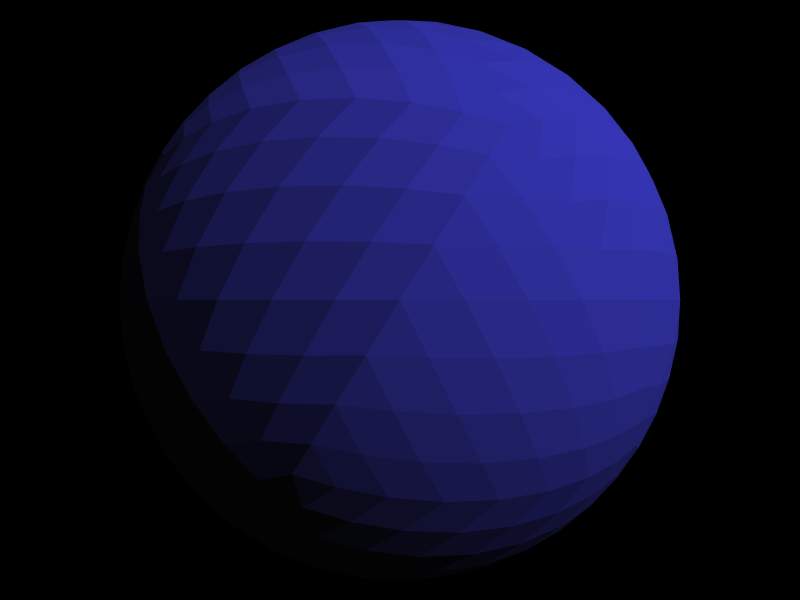
\includegraphics[scale=0.6]{img/flat_shading_crop.png}
\caption{Phongin valaistusmalli ilman spekulaaria termiä tasaisella varjostuksella.}
\label{fig:Tasainen_varjostus}
\end{figure}

\subsection{Gouraudin varjostus}
Gouraudin varjostus~\cite{Gouraud} on Henri Gouraudin vuonna 1971 kehittämä varjostusmenetelmä joka perustuu lineaariseen interpolointiin. Motivaatio Gouraudin varjostuksen kehitykseen syntyi tasaisen varjostuksen ongelmista kaarevien pintojen yhteydessä. Ensimmäiset ratkaisut kaarevien pintojen mallinnukseen perustuivat monikulmioverkkoihin, jotka koostuivat suuresta määrästä pieniä monikulmioita. Tällaisilla malleilla ja tasaisella varjostuksella luoduissa kuvissa nähdään selkeästi monikulmioiden välisten rajojen korostuminen.

Gouraud toteaa monikulmiorajojen korostumisen kappaleen pinnalla johtuvan ihmissilmän verkkokalvon neuronien vaikutuksista viereisiin neuroneihin. Tätä vaikutusta kutsutaan lateraaliseksi inhibitioksi, ja se aiheuttaa pintojen välisten intensiteettierojen korostumista~\cite[s. 29]{Glassner}. Ilmiön voi helposti huomata esimerkiksi Machin raidoiksi (Mach band effect) kutsutussa optisessa harhassa, missä tasaväriset palkit näyttävät tummemmilta kirkkaan palkin vieressä ja vastaavasti kirkkaammilta tumman palkin vieressä.

Gouraudin mukaan eräs ratkaisu monikulmiorajojen häivytykseen on monikulmioiden välisten värierojen pienentäminen monikulmiomäärän lisäyksellä. Hän kuitenkin totetaa tämän epäkäytännölliseksi tallennustilan ja aikavaatimusten nousun takia.

Tehokkaampi ratkaisu on seuraavaksi esiteltävä Gouraudin varjostus, joka säilyttää alkuperäisen kappaletta mallintavan monikulmioverkon. Siinä valaistusyhtälö evaluoidaan käyttäen monikulmion kulmapistenormaaleja ja interpoloidaan lineaarisesti monikulmion sisälle jääville pisteille. Gouraudin alkuperäisessä artikkelissa varjostus on esitelty käyttäen nelikulmiota, mutta tässä menetelmää sovelletaan kolmiolle.

Olkoot $A$, $B$ ja $C$ kolmion kulmapisteitä kaksiulotteisella tasolla ja $P$ piste tämän kolmion sisällä. Olkoon lisäksi $D$ pisteen $P$ y-koordinaatin määrittämä jakopiste sivulla $AC$ ja $E$ vastaava jakopiste sivulla $BC$. Tämä esitetään kuvassa~\ref{fig:Gouraud_interpolointi}.

\begin{figure}[h]
\centering
\begin{tikzpicture}[line cap=round,line join=round,>=triangle 45,x=1.0cm,y=1.0cm]
\clip(-3.0, -0.5) rectangle (3.0, 2.5);

\coordinate (A) at (-2.5, 0.0);
\coordinate (B) at (2.5, 0.0);
\coordinate (C) at (0.0, 2.0);
\coordinate (P) at (0.0, 1.0);

\draw[-] (A) -- (B);
\draw[-] (B) -- (C);
\draw[-] (C) -- (A);

\draw[red,-] (-2.0, 1.0) -- (2.0, 1.0);

\fill[black] (P) circle[radius=2pt];
\fill[black] (1.25, 1.0) circle[radius=2pt];
\fill[black] (-1.25, 1.0) circle[radius=2pt];

\begin{normalsize}
\draw[color=black] (-2.5, -0.3) node {$A$};
\draw[color=black] (2.5, -0.3) node {$B$};
\draw[color=black] (0.0, 2.2) node {$C$};

\draw[color=black] (0.0, 0.7) node {$P$};

\draw[color=black] (-1.2, 0.7) node {$D$};
\draw[color=black] (1.2, 0.7) node {$E$};
\end{normalsize}

\end{tikzpicture}
\caption{Gouraudin varjostuksen interpolointi.}
\label{fig:Gouraud_interpolointi}
\end{figure}

Merkitään $\alpha = \frac{\left|AD\right|}{\left|AC\right|}$ ja $\beta = \frac{\left|BE\right|}{\left|BC\right|}$, missä merkintä $\left|XY\right|$ tarkoittaa sivun $XY$ pituutta. Olkoot $S_A$, $S_B$, $S_C$ kulmapisteiden $A$, $B$ ja $C$ valaistusarvot. Pisteiden D ja E valaistusarvot $S_D$ ja $S_E$ voidaan nyt laskea interpoloimalla kaavoilla
\begin{align*}
& S_D = (1 - \alpha)S_A + \alpha S_C\\
& S_E = (1 - \beta)S_B + \beta S_C\,.
\end{align*}

Kun asetetaan $\gamma = \frac{\left|DP\right|}{\left|DE\right|}$, voidaan pisteen P interpoloitu valaistusarvo $S_P$ laskea kaavalla
\begin{align*}
S_P = (1 - \gamma)S_D + \gamma S_E\,.
\end{align*}

Kuvasta~\ref{fig:Gouraudin_varjostus} nähdään, että Gouraudin varjostus soveltuu hyvin mattapinnoille. Se tuottaa tasaista varjostusta sulavamman väriliukuman pinnan monikulmioiden välille ja häivyttää kappaletta mallintavan monikulmioverkon.

\begin{figure}[h]
\centering
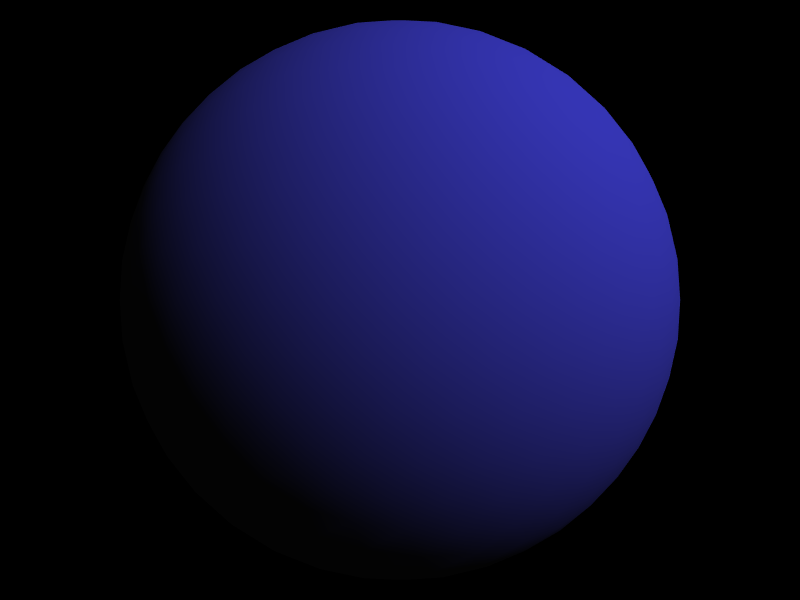
\includegraphics[scale=0.6]{img/gouraud_ambient_diff_crop.png}
\caption{Phongin valaistusmalli ilman spekulaaria termiä Gouraudin varjostuksella.}
\label{fig:Gouraudin_varjostus}
\end{figure}

Nykyaikaisilla näytönohjaimilla Gouraudin varjostus toteutetaan kulmapistevarjostimilla liittämällä jokaiseen kulmapisteeseen kulmapistenormaali, jolla valaistusyhtälö evaluoidaan. Kulmapistevarjostimen ohjelmakoodissa väriarvon sisältävä muuttuja määritellään interpoloitavaksi. Kun nyt pikselivarjostin suoritetaan näiden kulmapisteiden mallintamien monikulmioiden sisälle jääville pikseleille, välitetään interpoloitu väriarvo väripuskuriin, jolloin ollaan valmiita.

\subsection{Phongin varjostus}
\label{subsec:Phongin_varjostus}
Bui-Tuong Phong esitteli Phongin valaistusmallista kertovan artikkelin~\cite{Phong} yhteydessä myös uuden varjostustekniikan, jota nykyään kutsutaan Phongin varjostukseksi tai pikselikohtaiseksi varjostukseksi. Phongin varjostus häivyttää Gouraudin varjostuksessa havaittavan kappaleen monikulmioverkon korostumisen valaistusyhtälön vaihtuessa pinnan monikulmioiden välillä. Tämä Gouraudin varjostuksen heikkous nähdään etenkin spekulaarisesti heijastavilla pinnoilla, missä spekulaarisen heijastumisen huippukohdan muoto riippuu kappaletta mallintavista monikulmioista. Syy tähän on korkeimpien valaistusarvojen sijainti kappaleen kulmapistenormaalien kohdalla.

Gouraudin varjostuksen ongelmia havainnollistetaan kuvassa~\ref{fig:Gouraud_ongelma}. Kuvassa nähdään kuinka kappaleen kääntyessä spekulaarinen heijastus siirtyy kappaletta mallintavien monikulmioiden normaalivektoreiden ja valonlähteen välisen kulman muuttuessa.
\begin{figure}[h]
\centering
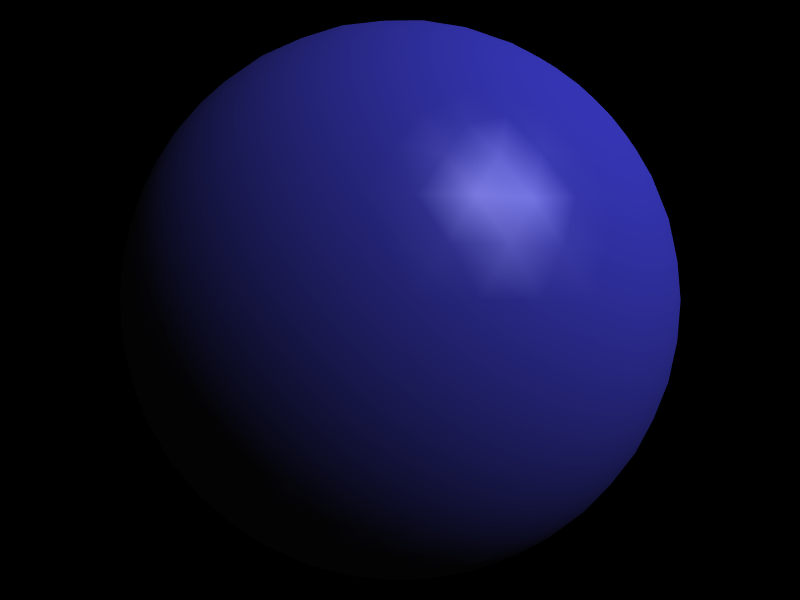
\includegraphics[width=0.49\textwidth]{img/gouraud_spec_1_crop.png}
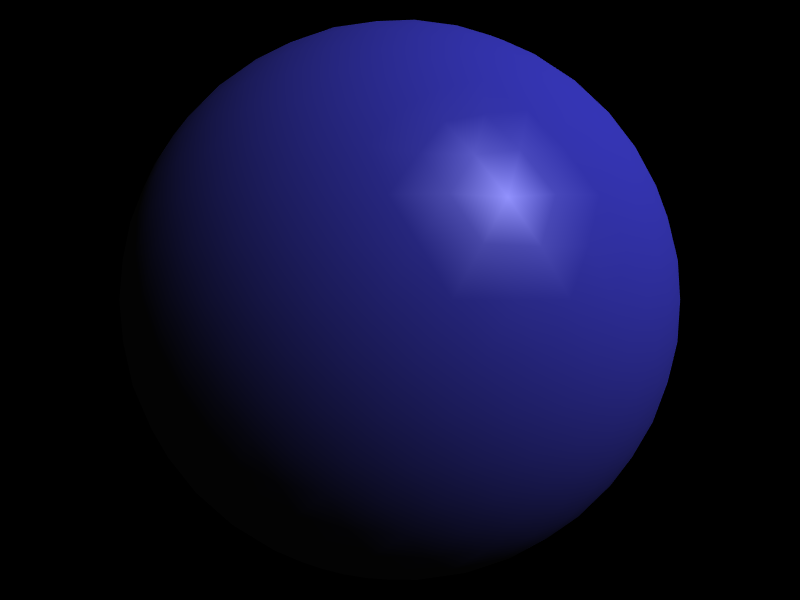
\includegraphics[width=0.49\textwidth]{img/gouraud_spec_2_crop.png}
\caption{Phongin valaistusmalli Gouraudin varjostuksella. Palloja on käännetty eri tavalla, jolloin spekulaarinen heijastuma näyttää eri muotoiselta. Vastaavaa ilmiötä ei tapahdu Phongin varjostuksella.}
\label{fig:Gouraud_ongelma}
\end{figure}

Phongin varjostus perustuu kulmapistenormaalien lineaariseen interpolointiin pikselikohtaisesti. Tässä esitellään kahden kulmapistenormaalin interpolointi monikulmion yhdellä sivulla. Olkoon $\vec{N_1}$ ja $\vec{N_2}$ monikulmion kulmapistenormaaleja sivulla $AB$, ja olkoon piste $P$ näiden välissä. Tätä havainnollistetaan kuvassa~\ref{fig:Phong_interpolointi}.
\begin{figure}[h]
\centering

\begin{tikzpicture}[line cap=round,line join=round,>=triangle 45,x=1.0cm,y=1.0cm]
\clip(-4.0, -0.7) rectangle (4.0, 2.5);

\coordinate (A) at (-2.0, 0.0);
\coordinate (B) at (2.0, 0);
\coordinate (P) at (0.0, 0.0);

\draw[-] (A) -- (P);
\draw[-] (P) -- (B);

\draw[->] (A) -- ($(A)!2cm!(-3.0, 0.5)$);
\draw[->] (B) -- ($(B)!2cm!(3.0, 0.5)$);
\draw[->] (P) -- ($(P)!2cm!(0.0, 1.0)$);

\draw[->] (-1.0, 0.0) -- ($(-1.0, 0.0)!2cm!(-1.5, 1.0)$);
\draw[->] (1.0, 0.0) -- ($(1.0, 0.0)!2cm!(1.5, 1.0)$);

\fill[black] (A) circle[radius=2pt];
\fill[black] (B) circle[radius=2pt];
\fill[black] (P) circle[radius=2pt];

\fill[black] (-1.0, 0.0) circle[radius=2pt];
\fill[black] (1.0, 0.0) circle[radius=2pt];

\begin{normalsize}
\draw[color=black] (-2.0, -0.5) node {$A$};
\draw[color=black] (2.0, -0.5) node {$B$};
\draw[color=black] (0.0, -0.5) node {$P$};

\draw[color=black] (-1.0, -0.5) node {$P_a$};
\draw[color=black] (1.0, -0.5) node {$P_b$};

\draw[color=black] (-3.5, 1.3) node {$\vec{N_1}$};
\draw[color=black] (3.5, 1.3) node {$\vec{N_2}$};
\draw[color=black] (0, 2.3) node {$\vec{N_I}$};
\end{normalsize}

\end{tikzpicture}
\caption{Kulmapistenormaalien interpolointi. Kuvassa $\vec{N_1}$ ja $\vec{N_2}$ ovat kulmapistenormaaleja ja $\vec{N_I}$ on näistä interpoloitu pisteen $P$ normaalivektori. Merkitsemättömät vektorit ovat normaalivektoreita pisteissä $P_a$ ja $P_b$.}
\label{fig:Phong_interpolointi}
\end{figure}
Merkitään $\alpha = \frac{\left|AP\right|}{\left|AB\right|}$, jolloin interpoloitu normaalivektori $\vec{N_I}$ voidaan laskea pisteelle $P$ sivulla AB kaavalla
\begin{align*}
\vec{N_I} = (1 - \alpha)\vec{N_1} + \alpha\vec{N_2}\,.
\end{align*}

Tätä menetelmää soveltamalla valaistusyhtälö voidaan evaluoida monikulmion sisälle jääville pikseleille käyttäen pikselikohtaisia normaalivektoreita, jotka on laskettu monikulmion kaikista kulmapistenormaaleista.

Nykyaikaisilla näytönohjaimilla Phongin varjostus toteutetaan merkitsemällä kulmapistevarjostimen ohjelmakoodissa kulmapistenormaalit interpoloitaviksi, jonka jälkeen valaistusyhtälö voidaan 
evaluoida pikselivarjostimella valmiiksi interpoloiduilla pikselikohtaisilla normaalivektoreilla.

Kuvasta~\ref{fig:Phong_valaistus} nähdään, että Phongin varjostus Gouraudin varjostusta todenmukaisemman lopputuloksen. Spekulaarisen heijastuman väriliukuma on pehmeämpi ja palloa mallintavaa monikulmioverkkoa ei voida enää havaita.

\begin{figure}[h]
\centering
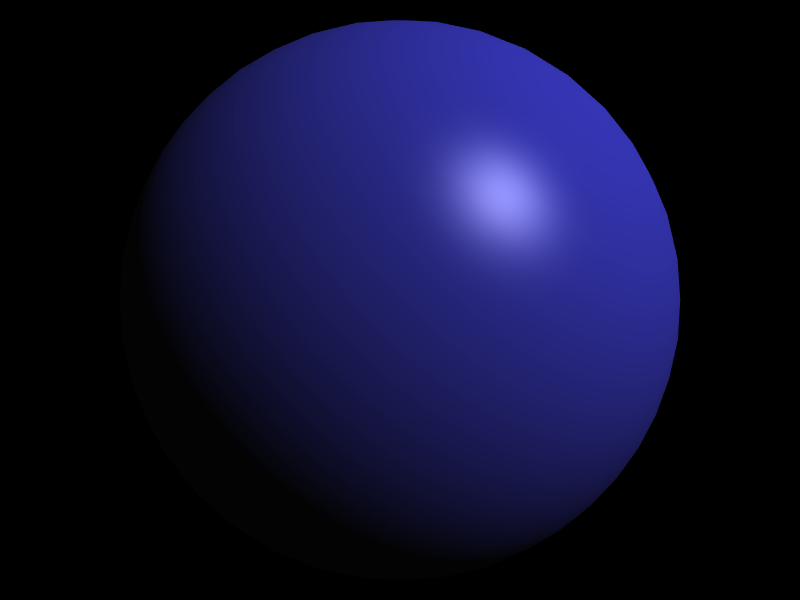
\includegraphics[scale=0.6]{img/phong_spec_crop.png}
\caption{Phongin valaistusmalli Phongin varjostuksella.}
\label{fig:Phong_valaistus}
\end{figure}

\newpage
\section{Yhteenveto}
Tässä tutkielmassa käsiteltiin reaaliaikaisen kolmiulotteisen tietokonegrafiikan ja valaistusmallinnuksen perusteet. Tutkielmassa huomattiin, kuinka tasaista varjostusta käytettäessä kuvat näyttävät auttamattoman keinotekoisilta selvästi näkyvän monikulmioverkon takia. Gouraudin varjostus parantaa kuvanlaatua huomattavasti ja soveltuu mattapinnoille. Gouraudin varjostuksen heikkous näkyy spekulaarisesti heijastavilla pinnoilla, joilla pintaa mallintava monikulmioverkko korostuu spekulaarisen heijastuman alueella. Lisäksi Gouraudin varjostus ei ole invariantti kun kappale liikkuu.

Phongin valaistusmalli yhdistettynä Phongin varjostukseen tarjoaa tehokkaan tavan mattapintojen ja spekulaaristi heijastavien pintojen likimääräiseen mallintaamiseen. Mikäli tehokkuutta tarvitaan lisää, voidaan käyttää hybridiratkaisua, missä mattapinnoille käytetään Gouraudin varjostusta.

Phongin valaistusmallia, Gouraudin varjostusta ja Phongin varjostusta käytetään edelleen yleisesti 3D-mallinnusohjelmissa, pelimoottoreissa ja piirtorajapinnoissa. Tasaisen varjostuksen käyttö nykyään rajoittuu lähinnä retrotyylisiin peleihin.

Tässä esitellyn valaistusmallin ja varjostustekniikoiden jälkeen on kehitetty tarkemmin fysiikkaan pohjautuvia malleja, jotka perustuvat esimerkiksi säteenjäljitykseen, mallinnettavan pinnan rakennetta kuvaaviin todennäköisyysjakaumiin, tai BRD-funktioihin (bidirectional reflectance distribution). Nämä laskennallisesti vaativammat valaistusmallit tuottavat todenmukaisempia kuvia laskentatehon kustannuksella. Vaikka osa näistä tekniikoista on jo käytössä, on esimerkiksi täysin säteenjäljitykseen perustuva renderöinti reaaliajassa toistaiseksi mahdotonta tämän hetken näytönohjaimilla.

\newpage

% --- References ---
%
% bibtex is used to generate the bibliography. The babplain style
% will generate numeric references (e.g. [1]) appropriate for theoretical
% computer science. If you need alphanumeric references (e.g [Tur90]), use
%
\bibliographystyle{babalpha-lf}
%
% instead.

%\bibliographystyle{babplain-lf}
\bibliography{references-fi}


% --- Appendices ---

% uncomment the following

% \newpage
% \appendix
% 
% \section{Esimerkkiliite}

\end{document}
